\documentclass[1p]{elsarticle_modified}
%\bibliographystyle{elsarticle-num}

%\usepackage[colorlinks]{hyperref}
%\usepackage{abbrmath_seonhwa} %\Abb, \Ascr, \Acal ,\Abf, \Afrak
\usepackage{amsfonts}
\usepackage{amssymb}
\usepackage{amsmath}
\usepackage{amsthm}
\usepackage{scalefnt}
\usepackage{amsbsy}
\usepackage{kotex}
\usepackage{caption}
\usepackage{subfig}
\usepackage{color}
\usepackage{graphicx}
\usepackage{xcolor} %% white, black, red, green, blue, cyan, magenta, yellow
\usepackage{float}
\usepackage{setspace}
\usepackage{hyperref}

\usepackage{tikz}
\usetikzlibrary{arrows}

\usepackage{multirow}
\usepackage{array} % fixed length table
\usepackage{hhline}

%%%%%%%%%%%%%%%%%%%%%
\makeatletter
\renewcommand*\env@matrix[1][\arraystretch]{%
	\edef\arraystretch{#1}%
	\hskip -\arraycolsep
	\let\@ifnextchar\new@ifnextchar
	\array{*\c@MaxMatrixCols c}}
\makeatother %https://tex.stackexchange.com/questions/14071/how-can-i-increase-the-line-spacing-in-a-matrix
%%%%%%%%%%%%%%%

\usepackage[normalem]{ulem}

\newcommand{\msout}[1]{\ifmmode\text{\sout{\ensuremath{#1}}}\else\sout{#1}\fi}
%SOURCE: \msout is \stkout macro in https://tex.stackexchange.com/questions/20609/strikeout-in-math-mode

\newcommand{\cancel}[1]{
	\ifmmode
	{\color{red}\msout{#1}}
	\else
	{\color{red}\sout{#1}}
	\fi
}

\newcommand{\add}[1]{
	{\color{blue}\uwave{#1}}
}

\newcommand{\replace}[2]{
	\ifmmode
	{\color{red}\msout{#1}}{\color{blue}\uwave{#2}}
	\else
	{\color{red}\sout{#1}}{\color{blue}\uwave{#2}}
	\fi
}

\newcommand{\Sol}{\mathcal{S}} %segment
\newcommand{\D}{D} %diagram
\newcommand{\A}{\mathcal{A}} %arc


%%%%%%%%%%%%%%%%%%%%%%%%%%%%%5 test

\def\sl{\operatorname{\textup{SL}}(2,\Cbb)}
\def\psl{\operatorname{\textup{PSL}}(2,\Cbb)}
\def\quan{\mkern 1mu \triangleright \mkern 1mu}

\theoremstyle{definition}
\newtheorem{thm}{Theorem}[section]
\newtheorem{prop}[thm]{Proposition}
\newtheorem{lem}[thm]{Lemma}
\newtheorem{ques}[thm]{Question}
\newtheorem{cor}[thm]{Corollary}
\newtheorem{defn}[thm]{Definition}
\newtheorem{exam}[thm]{Example}
\newtheorem{rmk}[thm]{Remark}
\newtheorem{alg}[thm]{Algorithm}

\newcommand{\I}{\sqrt{-1}}
\begin{document}

%\begin{frontmatter}
%
%\title{Boundary parabolic representations of knots up to 8 crossings}
%
%%% Group authors per affiliation:
%\author{Yunhi Cho} 
%\address{Department of Mathematics, University of Seoul, Seoul, Korea}
%\ead{yhcho@uos.ac.kr}
%
%
%\author{Seonhwa Kim} %\fnref{s_kim}}
%\address{Center for Geometry and Physics, Institute for Basic Science, Pohang, 37673, Korea}
%\ead{ryeona17@ibs.re.kr}
%
%\author{Hyuk Kim}
%\address{Department of Mathematical Sciences, Seoul National University, Seoul 08826, Korea}
%\ead{hyukkim@snu.ac.kr}
%
%\author{Seokbeom Yoon}
%\address{Department of Mathematical Sciences, Seoul National University, Seoul, 08826,  Korea}
%\ead{sbyoon15@snu.ac.kr}
%
%\begin{abstract}
%We find all boundary parabolic representation of knots up to 8 crossings.
%
%\end{abstract}
%\begin{keyword}
%    \MSC[2010] 57M25 
%\end{keyword}
%
%\end{frontmatter}

%\linenumbers
%\tableofcontents
%
\newcommand\colored[1]{\textcolor{white}{\rule[-0.35ex]{0.8em}{1.4ex}}\kern-0.8em\color{red} #1}%
%\newcommand\colored[1]{\textcolor{white}{ #1}\kern-2.17ex	\textcolor{white}{ #1}\kern-1.81ex	\textcolor{white}{ #1}\kern-2.15ex\color{red}#1	}

{\Large $\underline{12n_{0408}~(K12n_{0408})}$}

\setlength{\tabcolsep}{10pt}
\renewcommand{\arraystretch}{1.6}
\vspace{1cm}\begin{tabular}{m{100pt}>{\centering\arraybackslash}m{274pt}}
\multirow{5}{120pt}{
	\centering
	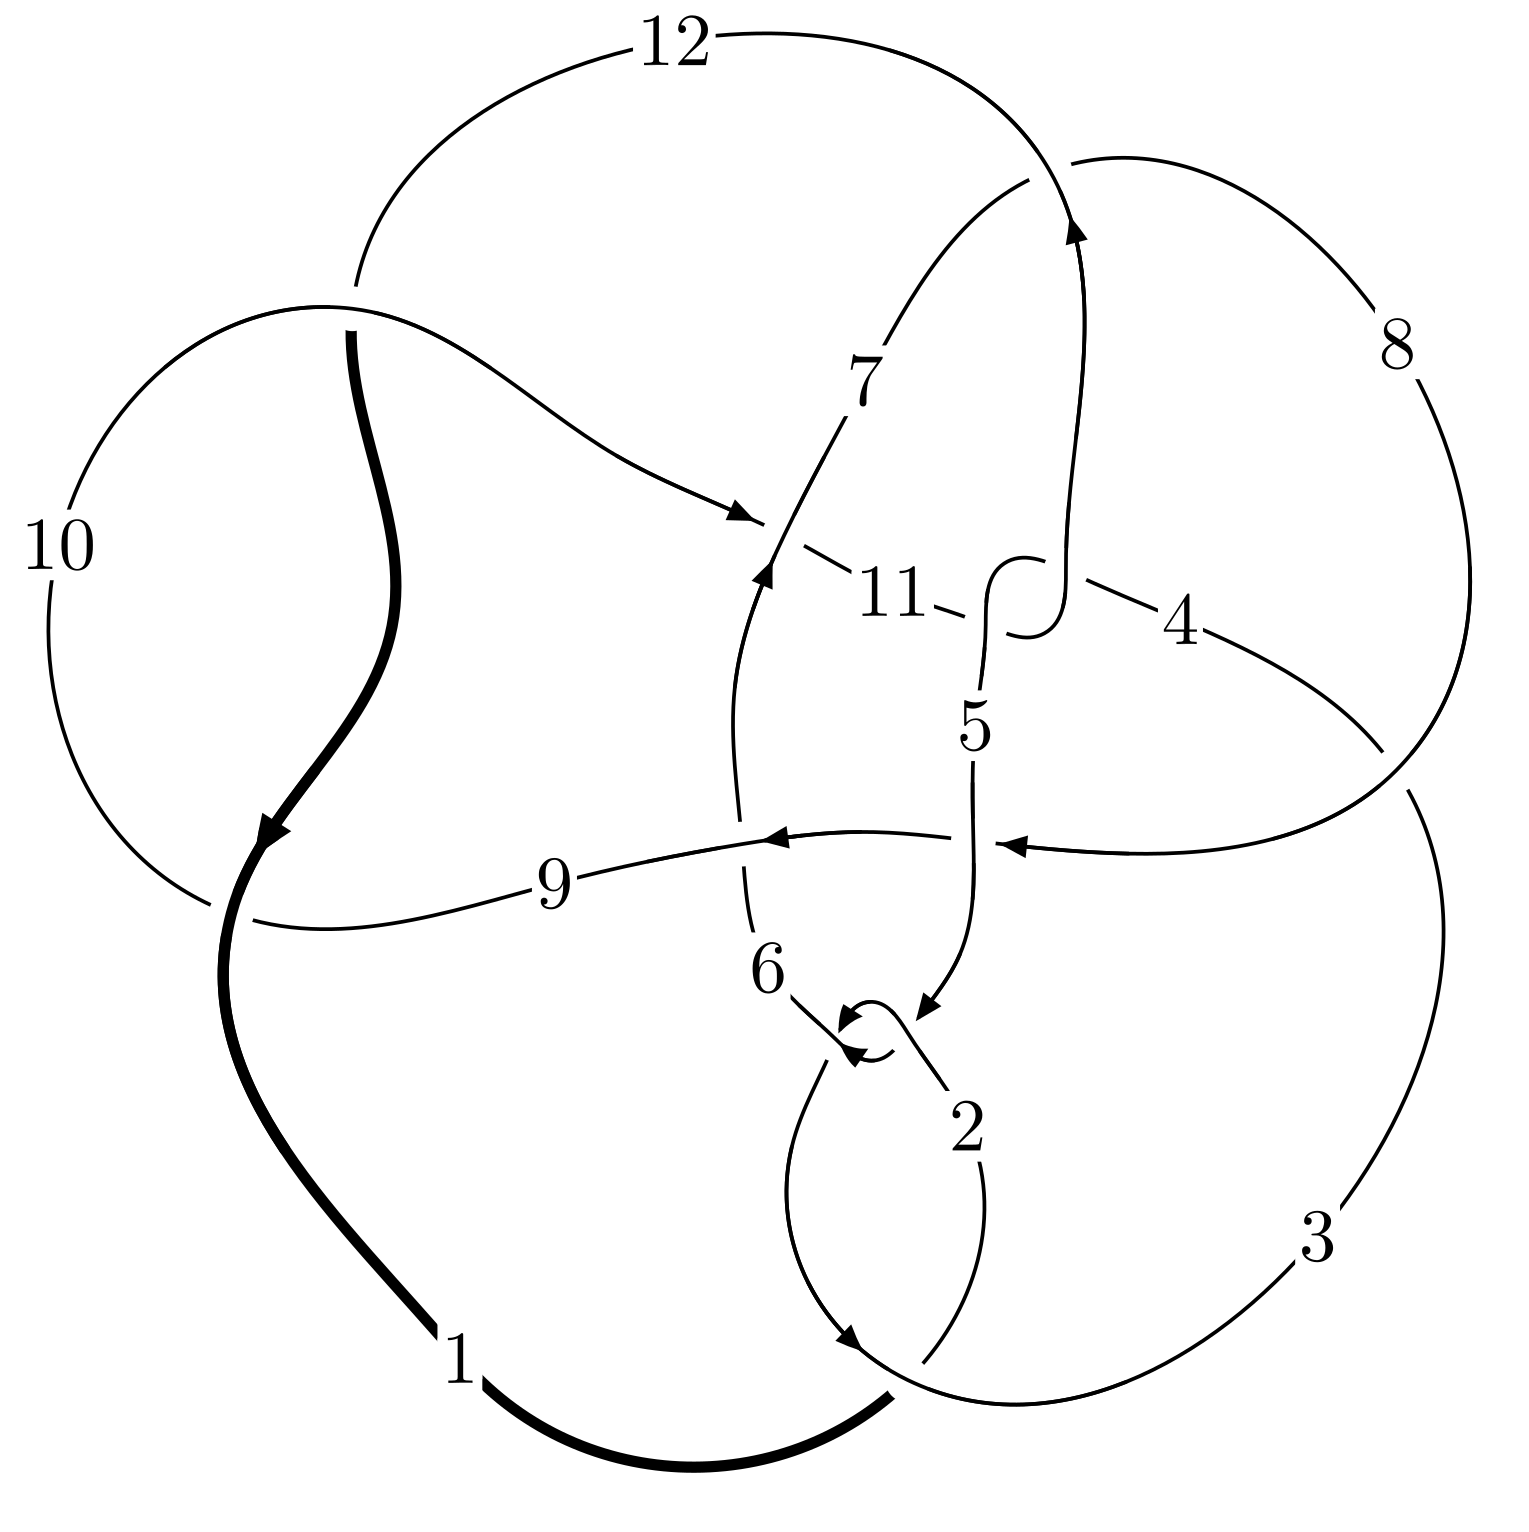
\includegraphics[width=112pt]{../../../GIT/diagram.site/Diagrams/png/2497_12n_0408.png}\\
\ \ \ A knot diagram\footnotemark}&
\allowdisplaybreaks
\textbf{Linearized knot diagam} \\
\cline{2-2}
 &
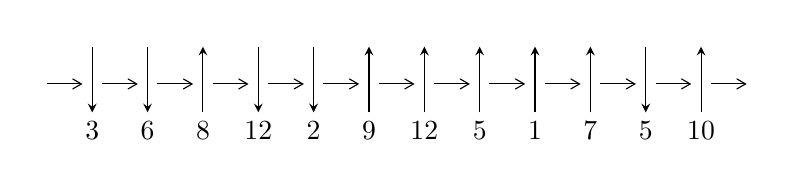
\begin{tikzpicture}[x=20pt, y=17pt]
	% nodes
	\node (C0) at (0, 0) {};
	\node (C1) at (1, 0) {};
	\node (C1U) at (1, +1) {};
	\node (C1D) at (1, -1) {3};

	\node (C2) at (2, 0) {};
	\node (C2U) at (2, +1) {};
	\node (C2D) at (2, -1) {6};

	\node (C3) at (3, 0) {};
	\node (C3U) at (3, +1) {};
	\node (C3D) at (3, -1) {8};

	\node (C4) at (4, 0) {};
	\node (C4U) at (4, +1) {};
	\node (C4D) at (4, -1) {12};

	\node (C5) at (5, 0) {};
	\node (C5U) at (5, +1) {};
	\node (C5D) at (5, -1) {2};

	\node (C6) at (6, 0) {};
	\node (C6U) at (6, +1) {};
	\node (C6D) at (6, -1) {9};

	\node (C7) at (7, 0) {};
	\node (C7U) at (7, +1) {};
	\node (C7D) at (7, -1) {12};

	\node (C8) at (8, 0) {};
	\node (C8U) at (8, +1) {};
	\node (C8D) at (8, -1) {5};

	\node (C9) at (9, 0) {};
	\node (C9U) at (9, +1) {};
	\node (C9D) at (9, -1) {1};

	\node (C10) at (10, 0) {};
	\node (C10U) at (10, +1) {};
	\node (C10D) at (10, -1) {7};

	\node (C11) at (11, 0) {};
	\node (C11U) at (11, +1) {};
	\node (C11D) at (11, -1) {5};

	\node (C12) at (12, 0) {};
	\node (C12U) at (12, +1) {};
	\node (C12D) at (12, -1) {10};
	\node (C13) at (13, 0) {};

	% arrows
	\draw[->,>={angle 60}]
	(C0) edge (C1) (C1) edge (C2) (C2) edge (C3) (C3) edge (C4) (C4) edge (C5) (C5) edge (C6) (C6) edge (C7) (C7) edge (C8) (C8) edge (C9) (C9) edge (C10) (C10) edge (C11) (C11) edge (C12) (C12) edge (C13) ;	\draw[->,>=stealth]
	(C1U) edge (C1D) (C2U) edge (C2D) (C3D) edge (C3U) (C4U) edge (C4D) (C5U) edge (C5D) (C6D) edge (C6U) (C7D) edge (C7U) (C8D) edge (C8U) (C9D) edge (C9U) (C10D) edge (C10U) (C11U) edge (C11D) (C12D) edge (C12U) ;
	\end{tikzpicture} \\
\hhline{~~} \\& 
\textbf{Solving Sequence} \\ \cline{2-2} 
 &
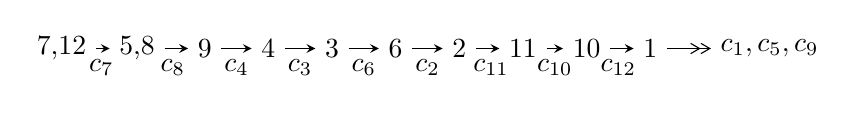
\begin{tikzpicture}[x=23pt, y=7pt]
	% node
	\node (A0) at (-1/8, 0) {7,12};
	\node (A1) at (17/16, 0) {5,8};
	\node (A2) at (17/8, 0) {9};
	\node (A3) at (25/8, 0) {4};
	\node (A4) at (33/8, 0) {3};
	\node (A5) at (41/8, 0) {6};
	\node (A6) at (49/8, 0) {2};
	\node (A7) at (57/8, 0) {11};
	\node (A8) at (65/8, 0) {10};
	\node (A9) at (73/8, 0) {1};
	\node (C1) at (1/2, -1) {$c_{7}$};
	\node (C2) at (13/8, -1) {$c_{8}$};
	\node (C3) at (21/8, -1) {$c_{4}$};
	\node (C4) at (29/8, -1) {$c_{3}$};
	\node (C5) at (37/8, -1) {$c_{6}$};
	\node (C6) at (45/8, -1) {$c_{2}$};
	\node (C7) at (53/8, -1) {$c_{11}$};
	\node (C8) at (61/8, -1) {$c_{10}$};
	\node (C9) at (69/8, -1) {$c_{12}$};
	\node (A10) at (11, 0) {$c_{1},c_{5},c_{9}$};

	% edge
	\draw[->,>=stealth]	
	(A0) edge (A1) (A1) edge (A2) (A2) edge (A3) (A3) edge (A4) (A4) edge (A5) (A5) edge (A6) (A6) edge (A7) (A7) edge (A8) (A8) edge (A9) ;
	\draw[->>,>={angle 60}]	
	(A9) edge (A10);
\end{tikzpicture} \\ 

\end{tabular} \\

\footnotetext{
The image of knot diagram is generated by the software ``\textbf{Draw programme}" developed by Andrew Bartholomew(\url{http://www.layer8.co.uk/maths/draw/index.htm\#Running-draw}), where we modified some parts for our purpose(\url{https://github.com/CATsTAILs/LinksPainter}).
}\phantom \\ \newline 
\centering \textbf{Ideals for irreducible components\footnotemark of $X_{\text{par}}$} 
 
\begin{align*}
I^u_{1}&=\langle 
3.32134\times10^{359} u^{70}-4.44408\times10^{359} u^{69}+\cdots+2.07193\times10^{364} b-6.03914\times10^{363},\\
\phantom{I^u_{1}}&\phantom{= \langle  }-2.44678\times10^{364} u^{70}+4.95782\times10^{364} u^{69}+\cdots+1.09626\times10^{368} a+4.70274\times10^{368},\\
\phantom{I^u_{1}}&\phantom{= \langle  }u^{71}-2 u^{70}+\cdots-50760 u+5291\rangle \\
I^u_{2}&=\langle 
-1.01666\times10^{17} u^{20}-3.63265\times10^{17} u^{19}+\cdots+1.76908\times10^{18} b-7.59833\times10^{17},\\
\phantom{I^u_{2}}&\phantom{= \langle  }-2.78942\times10^{18} u^{20}-2.28690\times10^{18} u^{19}+\cdots+5.30723\times10^{18} a-3.58565\times10^{18},\;u^{21}+u^{20}+\cdots+u+3\rangle \\
\\
\end{align*}
\raggedright * 2 irreducible components of $\dim_{\mathbb{C}}=0$, with total 92 representations.\\
\footnotetext{All coefficients of polynomials are rational numbers. But the coefficients are sometimes approximated in decimal forms when there is not enough margin.}
\newpage
\renewcommand{\arraystretch}{1}
\centering \section*{I. $I^u_{1}= \langle 3.32\times10^{359} u^{70}-4.44\times10^{359} u^{69}+\cdots+2.07\times10^{364} b-6.04\times10^{363},\;-2.45\times10^{364} u^{70}+4.96\times10^{364} u^{69}+\cdots+1.10\times10^{368} a+4.70\times10^{368},\;u^{71}-2 u^{70}+\cdots-50760 u+5291 \rangle$}
\flushleft \textbf{(i) Arc colorings}\\
\begin{tabular}{m{7pt} m{180pt} m{7pt} m{180pt} }
\flushright $a_{7}=$&$\begin{pmatrix}1\\0\end{pmatrix}$ \\
\flushright $a_{12}=$&$\begin{pmatrix}0\\u\end{pmatrix}$ \\
\flushright $a_{5}=$&$\begin{pmatrix}0.000223193 u^{70}-0.000452249 u^{69}+\cdots+29.0701 u-4.28980\\-0.0000160301 u^{70}+0.0000214489 u^{69}+\cdots+1.55560 u+0.291474\end{pmatrix}$ \\
\flushright $a_{8}=$&$\begin{pmatrix}1\\- u^2\end{pmatrix}$ \\
\flushright $a_{9}=$&$\begin{pmatrix}-0.000108414 u^{70}+0.000231215 u^{69}+\cdots-26.9057 u+3.05037\\0.0000349665 u^{70}-0.0000665424 u^{69}+\cdots-0.330042 u+0.239270\end{pmatrix}$ \\
\flushright $a_{4}=$&$\begin{pmatrix}0.000223193 u^{70}-0.000452249 u^{69}+\cdots+29.0701 u-4.28980\\-4.77057\times10^{-6} u^{70}-4.55792\times10^{-6} u^{69}+\cdots+3.03409 u+0.260456\end{pmatrix}$ \\
\flushright $a_{3}=$&$\begin{pmatrix}0.000239223 u^{70}-0.000473698 u^{69}+\cdots+27.5145 u-4.58128\\-4.53515\times10^{-6} u^{70}-5.71553\times10^{-6} u^{69}+\cdots+2.58027 u+0.316601\end{pmatrix}$ \\
\flushright $a_{6}=$&$\begin{pmatrix}-0.0000654430 u^{70}+0.000121036 u^{69}+\cdots+2.03966 u+1.27408\\-0.0000373474 u^{70}+0.0000850284 u^{69}+\cdots-4.95248 u+0.211483\end{pmatrix}$ \\
\flushright $a_{2}=$&$\begin{pmatrix}0.000128361 u^{70}-0.000267216 u^{69}+\cdots+30.3146 u-3.65679\\-0.0000243416 u^{70}+0.0000407389 u^{69}+\cdots-2.19710 u+0.550891\end{pmatrix}$ \\
\flushright $a_{11}=$&$\begin{pmatrix}-0.0000513840 u^{70}+0.0000471219 u^{69}+\cdots+9.13849 u-0.0700090\\-0.0000138702 u^{70}+0.0000242156 u^{69}+\cdots+7.00547 u-0.868044\end{pmatrix}$ \\
\flushright $a_{10}=$&$\begin{pmatrix}-0.0000375138 u^{70}+0.0000229063 u^{69}+\cdots+2.13303 u+0.798035\\-0.0000138702 u^{70}+0.0000242156 u^{69}+\cdots+7.00547 u-0.868044\end{pmatrix}$ \\
\flushright $a_{1}=$&$\begin{pmatrix}-0.000128274 u^{70}+0.000225121 u^{69}+\cdots+9.96795 u-1.80594\\-0.0000358515 u^{70}+0.0000911766 u^{69}+\cdots-9.35995 u+0.946339\end{pmatrix}$\\&\end{tabular}
\flushleft \textbf{(ii) Obstruction class $= -1$}\\~\\
\flushleft \textbf{(iii) Cusp Shapes $= 0.0000814784 u^{70}-0.000121110 u^{69}+\cdots-8.51691 u-4.14593$}\\~\\
\newpage\renewcommand{\arraystretch}{1}
\flushleft \textbf{(iv) u-Polynomials at the component}\newline \\
\begin{tabular}{m{50pt}|m{274pt}}
Crossings & \hspace{64pt}u-Polynomials at each crossing \\
\hline $$\begin{aligned}c_{1}\end{aligned}$$&$\begin{aligned}
&u^{71}+34 u^{70}+\cdots+99 u+1
\end{aligned}$\\
\hline $$\begin{aligned}c_{2},c_{5}\end{aligned}$$&$\begin{aligned}
&u^{71}+6 u^{70}+\cdots+3 u-1
\end{aligned}$\\
\hline $$\begin{aligned}c_{3}\end{aligned}$$&$\begin{aligned}
&u^{71}+3 u^{70}+\cdots+3403 u-821
\end{aligned}$\\
\hline $$\begin{aligned}c_{4},c_{11}\end{aligned}$$&$\begin{aligned}
&u^{71}+2 u^{70}+\cdots+8576 u-1849
\end{aligned}$\\
\hline $$\begin{aligned}c_{6}\end{aligned}$$&$\begin{aligned}
&u^{71}+18 u^{70}+\cdots-3847 u-341
\end{aligned}$\\
\hline $$\begin{aligned}c_{7}\end{aligned}$$&$\begin{aligned}
&u^{71}+2 u^{70}+\cdots-50760 u-5291
\end{aligned}$\\
\hline $$\begin{aligned}c_{8}\end{aligned}$$&$\begin{aligned}
&u^{71}-3 u^{70}+\cdots-921625 u-136291
\end{aligned}$\\
\hline $$\begin{aligned}c_{9},c_{12}\end{aligned}$$&$\begin{aligned}
&u^{71}+7 u^{70}+\cdots-836 u-53
\end{aligned}$\\
\hline $$\begin{aligned}c_{10}\end{aligned}$$&$\begin{aligned}
&u^{71}-4 u^{70}+\cdots-12683514 u-12102611
\end{aligned}$\\
\hline
\end{tabular}\\~\\
\newpage\renewcommand{\arraystretch}{1}
\flushleft \textbf{(v) Riley Polynomials at the component}\newline \\
\begin{tabular}{m{50pt}|m{274pt}}
Crossings & \hspace{64pt}Riley Polynomials at each crossing \\
\hline $$\begin{aligned}c_{1}\end{aligned}$$&$\begin{aligned}
&y^{71}+22 y^{70}+\cdots+7631 y-1
\end{aligned}$\\
\hline $$\begin{aligned}c_{2},c_{5}\end{aligned}$$&$\begin{aligned}
&y^{71}-34 y^{70}+\cdots+99 y-1
\end{aligned}$\\
\hline $$\begin{aligned}c_{3}\end{aligned}$$&$\begin{aligned}
&y^{71}+107 y^{70}+\cdots-25018129 y-674041
\end{aligned}$\\
\hline $$\begin{aligned}c_{4},c_{11}\end{aligned}$$&$\begin{aligned}
&y^{71}-96 y^{70}+\cdots+156138908 y-3418801
\end{aligned}$\\
\hline $$\begin{aligned}c_{6}\end{aligned}$$&$\begin{aligned}
&y^{71}+8 y^{70}+\cdots-3768041 y-116281
\end{aligned}$\\
\hline $$\begin{aligned}c_{7}\end{aligned}$$&$\begin{aligned}
&y^{71}+96 y^{70}+\cdots-99726602 y-27994681
\end{aligned}$\\
\hline $$\begin{aligned}c_{8}\end{aligned}$$&$\begin{aligned}
&y^{71}+31 y^{70}+\cdots-411466202141 y-18575236681
\end{aligned}$\\
\hline $$\begin{aligned}c_{9},c_{12}\end{aligned}$$&$\begin{aligned}
&y^{71}+51 y^{70}+\cdots+6292 y-2809
\end{aligned}$\\
\hline $$\begin{aligned}c_{10}\end{aligned}$$&$\begin{aligned}
&y^{71}+58 y^{70}+\cdots-4549217659521294 y-146473193017321
\end{aligned}$\\
\hline
\end{tabular}\\~\\
\newpage\flushleft \textbf{(vi) Complex Volumes and Cusp Shapes}
$$\begin{array}{c|c|c}  
\text{Solutions to }I^u_{1}& \I (\text{vol} + \sqrt{-1}CS) & \text{Cusp shape}\\
 \hline 
\begin{aligned}
u &= \phantom{-}0.580765 + 0.835800 I \\
a &= -0.292777 - 0.451256 I \\
b &= \phantom{-}0.282543 + 0.413279 I\end{aligned}
 & -4.96899 + 3.96926 I & \phantom{-0.000000 } 0. - 7.49324 I \\ \hline\begin{aligned}
u &= \phantom{-}0.580765 - 0.835800 I \\
a &= -0.292777 + 0.451256 I \\
b &= \phantom{-}0.282543 - 0.413279 I\end{aligned}
 & -4.96899 - 3.96926 I & \phantom{-0.000000 -}0. + 7.49324 I \\ \hline\begin{aligned}
u &= -0.788689 + 0.650257 I \\
a &= \phantom{-}0.878827 - 0.718311 I \\
b &= -0.098470 - 0.332871 I\end{aligned}
 & \phantom{-}1.02161 + 2.87191 I & \phantom{-0.000000 } 0 \\ \hline\begin{aligned}
u &= -0.788689 - 0.650257 I \\
a &= \phantom{-}0.878827 + 0.718311 I \\
b &= -0.098470 + 0.332871 I\end{aligned}
 & \phantom{-}1.02161 - 2.87191 I & \phantom{-0.000000 } 0 \\ \hline\begin{aligned}
u &= -1.102090 + 0.196980 I \\
a &= -0.565213 - 0.502463 I \\
b &= -0.181280 - 0.585679 I\end{aligned}
 & \phantom{-}1.32872 - 1.06319 I & \phantom{-0.000000 } 0 \\ \hline\begin{aligned}
u &= -1.102090 - 0.196980 I \\
a &= -0.565213 + 0.502463 I \\
b &= -0.181280 + 0.585679 I\end{aligned}
 & \phantom{-}1.32872 + 1.06319 I & \phantom{-0.000000 } 0 \\ \hline\begin{aligned}
u &= -0.644955 + 0.431962 I \\
a &= -0.131388 - 0.611300 I \\
b &= \phantom{-}1.44716 + 0.73868 I\end{aligned}
 & -1.87321 + 8.07778 I & -2.27368 - 4.02394 I \\ \hline\begin{aligned}
u &= -0.644955 - 0.431962 I \\
a &= -0.131388 + 0.611300 I \\
b &= \phantom{-}1.44716 - 0.73868 I\end{aligned}
 & -1.87321 - 8.07778 I & -2.27368 + 4.02394 I \\ \hline\begin{aligned}
u &= -1.219390 + 0.158809 I \\
a &= \phantom{-}0.605127 - 0.575176 I \\
b &= -0.018267 - 0.533663 I\end{aligned}
 & \phantom{-}0.46636 - 2.54570 I & \phantom{-0.000000 } 0 \\ \hline\begin{aligned}
u &= -1.219390 - 0.158809 I \\
a &= \phantom{-}0.605127 + 0.575176 I \\
b &= -0.018267 + 0.533663 I\end{aligned}
 & \phantom{-}0.46636 + 2.54570 I & \phantom{-0.000000 } 0\\
 \hline 
 \end{array}$$\newpage$$\begin{array}{c|c|c}  
\text{Solutions to }I^u_{1}& \I (\text{vol} + \sqrt{-1}CS) & \text{Cusp shape}\\
 \hline 
\begin{aligned}
u &= \phantom{-}0.338847 + 0.652992 I \\
a &= \phantom{-}2.05956 + 0.00269 I \\
b &= \phantom{-}0.322023 + 0.276626 I\end{aligned}
 & -2.65434 - 8.89707 I & -3.34744 + 5.99725 I \\ \hline\begin{aligned}
u &= \phantom{-}0.338847 - 0.652992 I \\
a &= \phantom{-}2.05956 - 0.00269 I \\
b &= \phantom{-}0.322023 - 0.276626 I\end{aligned}
 & -2.65434 + 8.89707 I & -3.34744 - 5.99725 I \\ \hline\begin{aligned}
u &= -0.413420 + 0.603171 I \\
a &= -1.19312 + 0.91314 I \\
b &= \phantom{-}0.013449 + 0.272129 I\end{aligned}
 & \phantom{-}2.09910 - 1.55037 I & \phantom{-}2.13059 + 4.88188 I \\ \hline\begin{aligned}
u &= -0.413420 - 0.603171 I \\
a &= -1.19312 - 0.91314 I \\
b &= \phantom{-}0.013449 - 0.272129 I\end{aligned}
 & \phantom{-}2.09910 + 1.55037 I & \phantom{-}2.13059 - 4.88188 I \\ \hline\begin{aligned}
u &= -0.206337 + 1.264600 I \\
a &= \phantom{-}0.87744 + 1.44981 I \\
b &= \phantom{-}0.97694 + 2.04446 I\end{aligned}
 & -7.83303 - 3.23562 I & \phantom{-0.000000 } 0 \\ \hline\begin{aligned}
u &= -0.206337 - 1.264600 I \\
a &= \phantom{-}0.87744 - 1.44981 I \\
b &= \phantom{-}0.97694 - 2.04446 I\end{aligned}
 & -7.83303 + 3.23562 I & \phantom{-0.000000 } 0 \\ \hline\begin{aligned}
u &= -0.495470 + 0.518548 I \\
a &= -0.309042 + 0.617419 I \\
b &= -1.36002 - 0.62813 I\end{aligned}
 & \phantom{-}0.29797 + 2.50456 I & \phantom{-}0.701081 - 0.103219 I \\ \hline\begin{aligned}
u &= -0.495470 - 0.518548 I \\
a &= -0.309042 - 0.617419 I \\
b &= -1.36002 + 0.62813 I\end{aligned}
 & \phantom{-}0.29797 - 2.50456 I & \phantom{-}0.701081 + 0.103219 I \\ \hline\begin{aligned}
u &= \phantom{-}0.659094 + 0.234693 I \\
a &= -0.688554 + 0.725722 I \\
b &= \phantom{-}0.061050 - 0.639663 I\end{aligned}
 & -1.59434 + 1.80020 I & \phantom{-}0.62667 - 4.98436 I \\ \hline\begin{aligned}
u &= \phantom{-}0.659094 - 0.234693 I \\
a &= -0.688554 - 0.725722 I \\
b &= \phantom{-}0.061050 + 0.639663 I\end{aligned}
 & -1.59434 - 1.80020 I & \phantom{-}0.62667 + 4.98436 I\\
 \hline 
 \end{array}$$\newpage$$\begin{array}{c|c|c}  
\text{Solutions to }I^u_{1}& \I (\text{vol} + \sqrt{-1}CS) & \text{Cusp shape}\\
 \hline 
\begin{aligned}
u &= \phantom{-}0.184729 + 0.633390 I \\
a &= -2.09854 + 0.37802 I \\
b &= -0.435861 - 0.070705 I\end{aligned}
 & -0.19378 - 3.46779 I & -1.36386 + 2.69751 I \\ \hline\begin{aligned}
u &= \phantom{-}0.184729 - 0.633390 I \\
a &= -2.09854 - 0.37802 I \\
b &= -0.435861 + 0.070705 I\end{aligned}
 & -0.19378 + 3.46779 I & -1.36386 - 2.69751 I \\ \hline\begin{aligned}
u &= \phantom{-}0.155035 + 1.339750 I \\
a &= \phantom{-}0.03561 - 1.62777 I \\
b &= -0.35185 - 2.24462 I\end{aligned}
 & -6.17756 + 4.77517 I & \phantom{-0.000000 } 0 \\ \hline\begin{aligned}
u &= \phantom{-}0.155035 - 1.339750 I \\
a &= \phantom{-}0.03561 + 1.62777 I \\
b &= -0.35185 + 2.24462 I\end{aligned}
 & -6.17756 - 4.77517 I & \phantom{-0.000000 } 0 \\ \hline\begin{aligned}
u &= -0.645433\phantom{ +0.000000I} \\
a &= -0.542319\phantom{ +0.000000I} \\
b &= -0.377916\phantom{ +0.000000I}\end{aligned}
 & \phantom{-}1.01771\phantom{ +0.000000I} & \phantom{-}11.3920\phantom{ +0.000000I} \\ \hline\begin{aligned}
u &= \phantom{-}1.270820 + 0.486913 I \\
a &= -0.482541 + 0.074369 I \\
b &= \phantom{-}0.453419 - 0.446420 I\end{aligned}
 & -1.12010 + 3.38645 I & \phantom{-0.000000 } 0 \\ \hline\begin{aligned}
u &= \phantom{-}1.270820 - 0.486913 I \\
a &= -0.482541 - 0.074369 I \\
b &= \phantom{-}0.453419 + 0.446420 I\end{aligned}
 & -1.12010 - 3.38645 I & \phantom{-0.000000 } 0 \\ \hline\begin{aligned}
u &= \phantom{-}1.027510 + 0.932024 I \\
a &= \phantom{-}0.338936 + 0.076836 I \\
b &= -0.448741 + 0.004535 I\end{aligned}
 & -4.73552 + 1.86861 I & \phantom{-0.000000 } 0 \\ \hline\begin{aligned}
u &= \phantom{-}1.027510 - 0.932024 I \\
a &= \phantom{-}0.338936 - 0.076836 I \\
b &= -0.448741 - 0.004535 I\end{aligned}
 & -4.73552 - 1.86861 I & \phantom{-0.000000 } 0 \\ \hline\begin{aligned}
u &= \phantom{-}0.045687 + 0.585291 I \\
a &= -0.191858 + 0.636762 I \\
b &= \phantom{-}1.130060 - 0.314443 I\end{aligned}
 & \phantom{-}0.83945 - 5.04601 I & -0.72754 + 7.42828 I\\
 \hline 
 \end{array}$$\newpage$$\begin{array}{c|c|c}  
\text{Solutions to }I^u_{1}& \I (\text{vol} + \sqrt{-1}CS) & \text{Cusp shape}\\
 \hline 
\begin{aligned}
u &= \phantom{-}0.045687 - 0.585291 I \\
a &= -0.191858 - 0.636762 I \\
b &= \phantom{-}1.130060 + 0.314443 I\end{aligned}
 & \phantom{-}0.83945 + 5.04601 I & -0.72754 - 7.42828 I \\ \hline\begin{aligned}
u &= -0.184861 + 0.554459 I \\
a &= -0.189001 - 0.545144 I \\
b &= -1.084770 + 0.040106 I\end{aligned}
 & \phantom{-}2.19151 - 0.19769 I & \phantom{-}2.21273 + 1.68853 I \\ \hline\begin{aligned}
u &= -0.184861 - 0.554459 I \\
a &= -0.189001 + 0.545144 I \\
b &= -1.084770 - 0.040106 I\end{aligned}
 & \phantom{-}2.19151 + 0.19769 I & \phantom{-}2.21273 - 1.68853 I \\ \hline\begin{aligned}
u &= \phantom{-}0.09305 + 1.45285 I \\
a &= -0.277047 + 1.109460 I \\
b &= -0.01604 + 1.70541 I\end{aligned}
 & -3.73297 - 1.70076 I & \phantom{-0.000000 } 0 \\ \hline\begin{aligned}
u &= \phantom{-}0.09305 - 1.45285 I \\
a &= -0.277047 - 1.109460 I \\
b &= -0.01604 - 1.70541 I\end{aligned}
 & -3.73297 + 1.70076 I & \phantom{-0.000000 } 0 \\ \hline\begin{aligned}
u &= \phantom{-}0.43800 + 1.46752 I \\
a &= \phantom{-}0.460286 - 0.948050 I \\
b &= -0.05146 - 1.72191 I\end{aligned}
 & -5.23559 + 3.76380 I & \phantom{-0.000000 } 0 \\ \hline\begin{aligned}
u &= \phantom{-}0.43800 - 1.46752 I \\
a &= \phantom{-}0.460286 + 0.948050 I \\
b &= -0.05146 + 1.72191 I\end{aligned}
 & -5.23559 - 3.76380 I & \phantom{-0.000000 } 0 \\ \hline\begin{aligned}
u &= \phantom{-}1.44469 + 0.67653 I \\
a &= \phantom{-}0.461376 + 0.000212 I \\
b &= -0.610829 + 0.359999 I\end{aligned}
 & -2.82185 + 8.13246 I & \phantom{-0.000000 } 0 \\ \hline\begin{aligned}
u &= \phantom{-}1.44469 - 0.67653 I \\
a &= \phantom{-}0.461376 - 0.000212 I \\
b &= -0.610829 - 0.359999 I\end{aligned}
 & -2.82185 - 8.13246 I & \phantom{-0.000000 } 0 \\ \hline\begin{aligned}
u &= \phantom{-}0.222485 + 0.329255 I \\
a &= -0.22314 - 2.06764 I \\
b &= \phantom{-}0.103952 + 0.761599 I\end{aligned}
 & -3.63364 - 2.57307 I & -2.03072 + 1.09466 I\\
 \hline 
 \end{array}$$\newpage$$\begin{array}{c|c|c}  
\text{Solutions to }I^u_{1}& \I (\text{vol} + \sqrt{-1}CS) & \text{Cusp shape}\\
 \hline 
\begin{aligned}
u &= \phantom{-}0.222485 - 0.329255 I \\
a &= -0.22314 + 2.06764 I \\
b &= \phantom{-}0.103952 - 0.761599 I\end{aligned}
 & -3.63364 + 2.57307 I & -2.03072 - 1.09466 I \\ \hline\begin{aligned}
u &= -0.036076 + 0.328318 I \\
a &= \phantom{-}2.77493 - 2.15222 I \\
b &= \phantom{-}0.956928 + 0.554431 I\end{aligned}
 & -6.09160 - 0.21690 I & -5.79568 - 0.48270 I \\ \hline\begin{aligned}
u &= -0.036076 - 0.328318 I \\
a &= \phantom{-}2.77493 + 2.15222 I \\
b &= \phantom{-}0.956928 - 0.554431 I\end{aligned}
 & -6.09160 + 0.21690 I & -5.79568 + 0.48270 I \\ \hline\begin{aligned}
u &= \phantom{-}0.14109 + 1.71542 I \\
a &= -0.103585 - 0.983039 I \\
b &= \phantom{-}0.41054 - 1.70085 I\end{aligned}
 & -8.85568 - 1.19614 I & \phantom{-0.000000 } 0 \\ \hline\begin{aligned}
u &= \phantom{-}0.14109 - 1.71542 I \\
a &= -0.103585 + 0.983039 I \\
b &= \phantom{-}0.41054 + 1.70085 I\end{aligned}
 & -8.85568 + 1.19614 I & \phantom{-0.000000 } 0 \\ \hline\begin{aligned}
u &= \phantom{-}0.50453 + 1.64767 I \\
a &= -0.021638 + 1.079040 I \\
b &= -0.31773 + 1.57830 I\end{aligned}
 & -11.19700 + 2.71939 I & \phantom{-0.000000 } 0 \\ \hline\begin{aligned}
u &= \phantom{-}0.50453 - 1.64767 I \\
a &= -0.021638 - 1.079040 I \\
b &= -0.31773 - 1.57830 I\end{aligned}
 & -11.19700 - 2.71939 I & \phantom{-0.000000 } 0 \\ \hline\begin{aligned}
u &= -0.33964 + 1.69087 I \\
a &= -0.270789 - 0.811108 I \\
b &= \phantom{-}0.63080 - 1.85770 I\end{aligned}
 & -8.42379 - 1.34719 I & \phantom{-0.000000 } 0 \\ \hline\begin{aligned}
u &= -0.33964 - 1.69087 I \\
a &= -0.270789 + 0.811108 I \\
b &= \phantom{-}0.63080 + 1.85770 I\end{aligned}
 & -8.42379 + 1.34719 I & \phantom{-0.000000 } 0 \\ \hline\begin{aligned}
u &= -0.38005 + 1.74334 I \\
a &= -0.004059 + 1.047000 I \\
b &= -0.14824 + 1.70632 I\end{aligned}
 & -4.48823 - 4.63881 I & \phantom{-0.000000 } 0\\
 \hline 
 \end{array}$$\newpage$$\begin{array}{c|c|c}  
\text{Solutions to }I^u_{1}& \I (\text{vol} + \sqrt{-1}CS) & \text{Cusp shape}\\
 \hline 
\begin{aligned}
u &= -0.38005 - 1.74334 I \\
a &= -0.004059 - 1.047000 I \\
b &= -0.14824 - 1.70632 I\end{aligned}
 & -4.48823 + 4.63881 I & \phantom{-0.000000 } 0 \\ \hline\begin{aligned}
u &= \phantom{-}0.144380 + 0.082580 I \\
a &= -2.20673 + 2.28717 I \\
b &= \phantom{-}0.462774 - 0.516661 I\end{aligned}
 & -1.49223 + 0.50005 I & -5.24006 - 0.19978 I \\ \hline\begin{aligned}
u &= \phantom{-}0.144380 - 0.082580 I \\
a &= -2.20673 - 2.28717 I \\
b &= \phantom{-}0.462774 + 0.516661 I\end{aligned}
 & -1.49223 - 0.50005 I & -5.24006 + 0.19978 I \\ \hline\begin{aligned}
u &= \phantom{-}0.20850 + 1.82203 I \\
a &= \phantom{-}0.081777 + 1.082370 I \\
b &= \phantom{-}0.40590 + 2.02173 I\end{aligned}
 & -15.0313 + 6.8617 I & \phantom{-0.000000 } 0 \\ \hline\begin{aligned}
u &= \phantom{-}0.20850 - 1.82203 I \\
a &= \phantom{-}0.081777 - 1.082370 I \\
b &= \phantom{-}0.40590 - 2.02173 I\end{aligned}
 & -15.0313 - 6.8617 I & \phantom{-0.000000 } 0 \\ \hline\begin{aligned}
u &= \phantom{-}0.45176 + 1.83563 I \\
a &= \phantom{-}0.042954 - 1.024460 I \\
b &= -0.39692 - 2.03294 I\end{aligned}
 & -8.94192 + 10.31780 I & \phantom{-0.000000 } 0 \\ \hline\begin{aligned}
u &= \phantom{-}0.45176 - 1.83563 I \\
a &= \phantom{-}0.042954 + 1.024460 I \\
b &= -0.39692 + 2.03294 I\end{aligned}
 & -8.94192 - 10.31780 I & \phantom{-0.000000 } 0 \\ \hline\begin{aligned}
u &= -0.50536 + 1.86907 I \\
a &= -0.039033 - 1.008760 I \\
b &= \phantom{-}0.17763 - 1.71497 I\end{aligned}
 & -6.53854 - 9.81945 I & \phantom{-0.000000 } 0 \\ \hline\begin{aligned}
u &= -0.50536 - 1.86907 I \\
a &= -0.039033 + 1.008760 I \\
b &= \phantom{-}0.17763 + 1.71497 I\end{aligned}
 & -6.53854 + 9.81945 I & \phantom{-0.000000 } 0 \\ \hline\begin{aligned}
u &= -0.09707 + 1.98496 I \\
a &= \phantom{-}0.057879 - 0.937148 I \\
b &= \phantom{-}0.14717 - 1.77957 I\end{aligned}
 & -9.48997 - 2.54176 I & \phantom{-0.000000 } 0\\
 \hline 
 \end{array}$$\newpage$$\begin{array}{c|c|c}  
\text{Solutions to }I^u_{1}& \I (\text{vol} + \sqrt{-1}CS) & \text{Cusp shape}\\
 \hline 
\begin{aligned}
u &= -0.09707 - 1.98496 I \\
a &= \phantom{-}0.057879 + 0.937148 I \\
b &= \phantom{-}0.14717 + 1.77957 I\end{aligned}
 & -9.48997 + 2.54176 I & \phantom{-0.000000 } 0 \\ \hline\begin{aligned}
u &= \phantom{-}0.49330 + 1.95007 I \\
a &= -0.031263 + 0.967843 I \\
b &= \phantom{-}0.39373 + 2.03998 I\end{aligned}
 & -11.4134 + 16.1003 I & \phantom{-0.000000 } 0 \\ \hline\begin{aligned}
u &= \phantom{-}0.49330 - 1.95007 I \\
a &= -0.031263 - 0.967843 I \\
b &= \phantom{-}0.39373 - 2.03998 I\end{aligned}
 & -11.4134 - 16.1003 I & \phantom{-0.000000 } 0 \\ \hline\begin{aligned}
u &= -0.67907 + 1.94610 I \\
a &= \phantom{-}0.247969 + 0.639732 I \\
b &= -0.72680 + 2.09501 I\end{aligned}
 & -10.02920 - 5.17198 I & \phantom{-0.000000 } 0 \\ \hline\begin{aligned}
u &= -0.67907 - 1.94610 I \\
a &= \phantom{-}0.247969 - 0.639732 I \\
b &= -0.72680 - 2.09501 I\end{aligned}
 & -10.02920 + 5.17198 I & \phantom{-0.000000 } 0 \\ \hline\begin{aligned}
u &= \phantom{-}0.34344 + 2.04434 I \\
a &= -0.025252 + 0.944078 I \\
b &= -0.25012 + 1.70609 I\end{aligned}
 & -11.65100 - 4.31172 I & \phantom{-0.000000 } 0 \\ \hline\begin{aligned}
u &= \phantom{-}0.34344 - 2.04434 I \\
a &= -0.025252 - 0.944078 I \\
b &= -0.25012 - 1.70609 I\end{aligned}
 & -11.65100 + 4.31172 I & \phantom{-0.000000 } 0 \\ \hline\begin{aligned}
u &= \phantom{-}0.00982 + 2.14846 I \\
a &= \phantom{-}0.009145 - 0.765336 I \\
b &= \phantom{-}0.24624 - 1.99478 I\end{aligned}
 & -9.17505 - 2.02606 I & \phantom{-0.000000 } 0 \\ \hline\begin{aligned}
u &= \phantom{-}0.00982 - 2.14846 I \\
a &= \phantom{-}0.009145 + 0.765336 I \\
b &= \phantom{-}0.24624 + 1.99478 I\end{aligned}
 & -9.17505 + 2.02606 I & \phantom{-0.000000 } 0 \\ \hline\begin{aligned}
u &= -0.34232 + 2.31471 I \\
a &= \phantom{-}0.089041 + 0.645209 I \\
b &= -0.43595 + 2.20178 I\end{aligned}
 & -10.43290 + 1.02273 I & \phantom{-0.000000 } 0\\
 \hline 
 \end{array}$$\newpage$$\begin{array}{c|c|c}  
\text{Solutions to }I^u_{1}& \I (\text{vol} + \sqrt{-1}CS) & \text{Cusp shape}\\
 \hline 
\begin{aligned}
u &= -0.34232 - 2.31471 I \\
a &= \phantom{-}0.089041 - 0.645209 I \\
b &= -0.43595 - 2.20178 I\end{aligned}
 & -10.43290 - 1.02273 I & \phantom{-0.000000 } 0\\
 \hline 
 \end{array}$$\newpage\newpage\renewcommand{\arraystretch}{1}
\centering \section*{II. $I^u_{2}= \langle -1.02\times10^{17} u^{20}-3.63\times10^{17} u^{19}+\cdots+1.77\times10^{18} b-7.60\times10^{17},\;-2.79\times10^{18} u^{20}-2.29\times10^{18} u^{19}+\cdots+5.31\times10^{18} a-3.59\times10^{18},\;u^{21}+u^{20}+\cdots+u+3 \rangle$}
\flushleft \textbf{(i) Arc colorings}\\
\begin{tabular}{m{7pt} m{180pt} m{7pt} m{180pt} }
\flushright $a_{7}=$&$\begin{pmatrix}1\\0\end{pmatrix}$ \\
\flushright $a_{12}=$&$\begin{pmatrix}0\\u\end{pmatrix}$ \\
\flushright $a_{5}=$&$\begin{pmatrix}0.525589 u^{20}+0.430902 u^{19}+\cdots-3.87934 u+0.675616\\0.0574685 u^{20}+0.205341 u^{19}+\cdots-0.674948 u+0.429508\end{pmatrix}$ \\
\flushright $a_{8}=$&$\begin{pmatrix}1\\- u^2\end{pmatrix}$ \\
\flushright $a_{9}=$&$\begin{pmatrix}-0.639678 u^{20}-0.519629 u^{19}+\cdots+3.71273 u+0.974140\\-0.198195 u^{20}-0.215992 u^{19}+\cdots+1.23162 u-0.765561\end{pmatrix}$ \\
\flushright $a_{4}=$&$\begin{pmatrix}0.525589 u^{20}+0.430902 u^{19}+\cdots-3.87934 u+0.675616\\0.0333158 u^{20}+0.195091 u^{19}+\cdots+0.807132 u+0.145445\end{pmatrix}$ \\
\flushright $a_{3}=$&$\begin{pmatrix}0.468121 u^{20}+0.225560 u^{19}+\cdots-3.20440 u+0.246108\\0.0242084 u^{20}+0.247013 u^{19}+\cdots+0.486854 u-0.298173\end{pmatrix}$ \\
\flushright $a_{6}=$&$\begin{pmatrix}0.243288 u^{20}+0.0876454 u^{19}+\cdots-1.24949 u-0.505262\\0.414187 u^{20}+0.520712 u^{19}+\cdots-2.89587 u-0.0634637\end{pmatrix}$ \\
\flushright $a_{2}=$&$\begin{pmatrix}0.296423 u^{20}+0.0723191 u^{19}+\cdots-1.42924 u-0.964066\\0.265495 u^{20}+0.472573 u^{19}+\cdots-1.61833 u-0.682384\end{pmatrix}$ \\
\flushright $a_{11}=$&$\begin{pmatrix}-0.327392 u^{20}-0.257031 u^{19}+\cdots-1.30080 u-0.247004\\0.0570984 u^{20}+0.205606 u^{19}+\cdots-0.525634 u-1.70795\end{pmatrix}$ \\
\flushright $a_{10}=$&$\begin{pmatrix}-0.384491 u^{20}-0.462637 u^{19}+\cdots-0.775171 u+1.46095\\0.0570984 u^{20}+0.205606 u^{19}+\cdots-0.525634 u-1.70795\end{pmatrix}$ \\
\flushright $a_{1}=$&$\begin{pmatrix}0.717824 u^{20}+0.795971 u^{19}+\cdots-5.55816 u-2.12761\\-0.148508 u^{20}-0.169556 u^{19}+\cdots+2.76505 u+1.17130\end{pmatrix}$\\&\end{tabular}
\flushleft \textbf{(ii) Obstruction class $= 1$}\\~\\
\flushleft \textbf{(iii) Cusp Shapes $= -\frac{2705003835397264499}{1769077763043388471} u^{20}-\frac{2258477885563098772}{1769077763043388471} u^{19}+\cdots+\frac{11494347706283494126}{1769077763043388471} u+\frac{15960298128399919686}{1769077763043388471}$}\\~\\
\newpage\renewcommand{\arraystretch}{1}
\flushleft \textbf{(iv) u-Polynomials at the component}\newline \\
\begin{tabular}{m{50pt}|m{274pt}}
Crossings & \hspace{64pt}u-Polynomials at each crossing \\
\hline $$\begin{aligned}c_{1}\end{aligned}$$&$\begin{aligned}
&u^{21}-11 u^{20}+\cdots+88 u-9
\end{aligned}$\\
\hline $$\begin{aligned}c_{2}\end{aligned}$$&$\begin{aligned}
&u^{21}+u^{20}+\cdots-4 u-3
\end{aligned}$\\
\hline $$\begin{aligned}c_{3}\end{aligned}$$&$\begin{aligned}
&u^{21}-2 u^{20}+\cdots+10 u+5
\end{aligned}$\\
\hline $$\begin{aligned}c_{4}\end{aligned}$$&$\begin{aligned}
&u^{21}- u^{20}+\cdots-3 u+1
\end{aligned}$\\
\hline $$\begin{aligned}c_{5}\end{aligned}$$&$\begin{aligned}
&u^{21}- u^{20}+\cdots-4 u+3
\end{aligned}$\\
\hline $$\begin{aligned}c_{6}\end{aligned}$$&$\begin{aligned}
&u^{21}+u^{20}+\cdots+8 u^2+1
\end{aligned}$\\
\hline $$\begin{aligned}c_{7}\end{aligned}$$&$\begin{aligned}
&u^{21}+u^{20}+\cdots+u+3
\end{aligned}$\\
\hline $$\begin{aligned}c_{8}\end{aligned}$$&$\begin{aligned}
&u^{21}+2 u^{20}+\cdots-8 u^2-1
\end{aligned}$\\
\hline $$\begin{aligned}c_{9}\end{aligned}$$&$\begin{aligned}
&u^{21}+6 u^{20}+\cdots+45 u+5
\end{aligned}$\\
\hline $$\begin{aligned}c_{10}\end{aligned}$$&$\begin{aligned}
&u^{21}+3 u^{20}+\cdots+7 u-1
\end{aligned}$\\
\hline $$\begin{aligned}c_{11}\end{aligned}$$&$\begin{aligned}
&u^{21}+u^{20}+\cdots-3 u-1
\end{aligned}$\\
\hline $$\begin{aligned}c_{12}\end{aligned}$$&$\begin{aligned}
&u^{21}-6 u^{20}+\cdots+45 u-5
\end{aligned}$\\
\hline
\end{tabular}\\~\\
\newpage\renewcommand{\arraystretch}{1}
\flushleft \textbf{(v) Riley Polynomials at the component}\newline \\
\begin{tabular}{m{50pt}|m{274pt}}
Crossings & \hspace{64pt}Riley Polynomials at each crossing \\
\hline $$\begin{aligned}c_{1}\end{aligned}$$&$\begin{aligned}
&y^{21}+13 y^{20}+\cdots+184 y-81
\end{aligned}$\\
\hline $$\begin{aligned}c_{2},c_{5}\end{aligned}$$&$\begin{aligned}
&y^{21}-11 y^{20}+\cdots+88 y-9
\end{aligned}$\\
\hline $$\begin{aligned}c_{3}\end{aligned}$$&$\begin{aligned}
&y^{21}+22 y^{20}+\cdots+840 y-25
\end{aligned}$\\
\hline $$\begin{aligned}c_{4},c_{11}\end{aligned}$$&$\begin{aligned}
&y^{21}-17 y^{20}+\cdots-3 y-1
\end{aligned}$\\
\hline $$\begin{aligned}c_{6}\end{aligned}$$&$\begin{aligned}
&y^{21}-5 y^{20}+\cdots-16 y-1
\end{aligned}$\\
\hline $$\begin{aligned}c_{7}\end{aligned}$$&$\begin{aligned}
&y^{21}+19 y^{20}+\cdots+115 y-9
\end{aligned}$\\
\hline $$\begin{aligned}c_{8}\end{aligned}$$&$\begin{aligned}
&y^{21}+6 y^{20}+\cdots-16 y-1
\end{aligned}$\\
\hline $$\begin{aligned}c_{9},c_{12}\end{aligned}$$&$\begin{aligned}
&y^{21}+14 y^{20}+\cdots+265 y-25
\end{aligned}$\\
\hline $$\begin{aligned}c_{10}\end{aligned}$$&$\begin{aligned}
&y^{21}+9 y^{20}+\cdots+7 y-1
\end{aligned}$\\
\hline
\end{tabular}\\~\\
\newpage\flushleft \textbf{(vi) Complex Volumes and Cusp Shapes}
$$\begin{array}{c|c|c}  
\text{Solutions to }I^u_{2}& \I (\text{vol} + \sqrt{-1}CS) & \text{Cusp shape}\\
 \hline 
\begin{aligned}
u &= -1.017760 + 0.164191 I \\
a &= \phantom{-}0.019420 - 0.728210 I \\
b &= -0.217020 - 0.758452 I\end{aligned}
 & \phantom{-}0.01218 - 1.44237 I & -3.57616 + 0.36303 I \\ \hline\begin{aligned}
u &= -1.017760 - 0.164191 I \\
a &= \phantom{-}0.019420 + 0.728210 I \\
b &= -0.217020 + 0.758452 I\end{aligned}
 & \phantom{-}0.01218 + 1.44237 I & -3.57616 - 0.36303 I \\ \hline\begin{aligned}
u &= -0.667983 + 0.500875 I \\
a &= \phantom{-}0.264507 - 0.993663 I \\
b &= -0.740886 - 0.591101 I\end{aligned}
 & \phantom{-}1.64283 + 4.02770 I & \phantom{-}3.16447 - 4.97726 I \\ \hline\begin{aligned}
u &= -0.667983 - 0.500875 I \\
a &= \phantom{-}0.264507 + 0.993663 I \\
b &= -0.740886 + 0.591101 I\end{aligned}
 & \phantom{-}1.64283 - 4.02770 I & \phantom{-}3.16447 + 4.97726 I \\ \hline\begin{aligned}
u &= \phantom{-}0.954936 + 0.692254 I \\
a &= \phantom{-}0.072870 - 0.298348 I \\
b &= -0.378423 - 0.311339 I\end{aligned}
 & -4.60032 + 2.49760 I & \phantom{-}0.02822 - 6.06015 I \\ \hline\begin{aligned}
u &= \phantom{-}0.954936 - 0.692254 I \\
a &= \phantom{-}0.072870 + 0.298348 I \\
b &= -0.378423 + 0.311339 I\end{aligned}
 & -4.60032 - 2.49760 I & \phantom{-}0.02822 + 6.06015 I \\ \hline\begin{aligned}
u &= -0.811685\phantom{ +0.000000I} \\
a &= \phantom{-}0.881305\phantom{ +0.000000I} \\
b &= \phantom{-}0.180005\phantom{ +0.000000I}\end{aligned}
 & \phantom{-}0.358951\phantom{ +0.000000I} & -3.34010\phantom{ +0.000000I} \\ \hline\begin{aligned}
u &= \phantom{-}0.755182 + 0.080789 I \\
a &= \phantom{-}0.423871 - 1.018030 I \\
b &= -1.089450 - 0.150699 I\end{aligned}
 & -0.92163 + 9.19955 I & \phantom{-}2.77433 - 8.25516 I \\ \hline\begin{aligned}
u &= \phantom{-}0.755182 - 0.080789 I \\
a &= \phantom{-}0.423871 + 1.018030 I \\
b &= -1.089450 + 0.150699 I\end{aligned}
 & -0.92163 - 9.19955 I & \phantom{-}2.77433 + 8.25516 I \\ \hline\begin{aligned}
u &= \phantom{-}0.311855 + 1.336120 I \\
a &= -0.607669 + 0.987511 I \\
b &= -0.69526 + 1.74117 I\end{aligned}
 & -7.42230 + 2.81144 I & -2.33733 + 0.74449 I\\
 \hline 
 \end{array}$$\newpage$$\begin{array}{c|c|c}  
\text{Solutions to }I^u_{2}& \I (\text{vol} + \sqrt{-1}CS) & \text{Cusp shape}\\
 \hline 
\begin{aligned}
u &= \phantom{-}0.311855 - 1.336120 I \\
a &= -0.607669 - 0.987511 I \\
b &= -0.69526 - 1.74117 I\end{aligned}
 & -7.42230 - 2.81144 I & -2.33733 - 0.74449 I \\ \hline\begin{aligned}
u &= -0.271251 + 1.356350 I \\
a &= -0.46017 - 1.35418 I \\
b &= \phantom{-}0.12651 - 1.96996 I\end{aligned}
 & -6.42306 - 4.13848 I & -5.49167 + 2.04959 I \\ \hline\begin{aligned}
u &= -0.271251 - 1.356350 I \\
a &= -0.46017 + 1.35418 I \\
b &= \phantom{-}0.12651 + 1.96996 I\end{aligned}
 & -6.42306 + 4.13848 I & -5.49167 - 2.04959 I \\ \hline\begin{aligned}
u &= -0.468317 + 0.327808 I \\
a &= -0.17804 + 1.48507 I \\
b &= \phantom{-}0.762786 + 0.342701 I\end{aligned}
 & \phantom{-}2.92449 - 0.74097 I & \phantom{-}7.31939 + 1.52438 I \\ \hline\begin{aligned}
u &= -0.468317 - 0.327808 I \\
a &= -0.17804 - 1.48507 I \\
b &= \phantom{-}0.762786 - 0.342701 I\end{aligned}
 & \phantom{-}2.92449 + 0.74097 I & \phantom{-}7.31939 - 1.52438 I \\ \hline\begin{aligned}
u &= \phantom{-}0.474570 + 0.190158 I \\
a &= -0.01766 + 1.77843 I \\
b &= \phantom{-}1.076620 + 0.036349 I\end{aligned}
 & \phantom{-}1.07014 + 3.68507 I & \phantom{-}5.59024 - 4.51475 I \\ \hline\begin{aligned}
u &= \phantom{-}0.474570 - 0.190158 I \\
a &= -0.01766 - 1.77843 I \\
b &= \phantom{-}1.076620 - 0.036349 I\end{aligned}
 & \phantom{-}1.07014 - 3.68507 I & \phantom{-}5.59024 + 4.51475 I \\ \hline\begin{aligned}
u &= -0.23006 + 2.10695 I \\
a &= -0.158253 - 0.739024 I \\
b &= \phantom{-}0.46119 - 1.91480 I\end{aligned}
 & -9.48831 - 0.32291 I & -3.90057 - 0.91919 I \\ \hline\begin{aligned}
u &= -0.23006 - 2.10695 I \\
a &= -0.158253 + 0.739024 I \\
b &= \phantom{-}0.46119 + 1.91480 I\end{aligned}
 & -9.48831 + 0.32291 I & -3.90057 + 0.91919 I \\ \hline\begin{aligned}
u &= \phantom{-}0.06467 + 2.12010 I \\
a &= \phantom{-}0.033800 + 0.726331 I \\
b &= -0.39606 + 1.95200 I\end{aligned}
 & -9.87219 - 3.28291 I & -3.90087 + 4.45768 I\\
 \hline 
 \end{array}$$\newpage$$\begin{array}{c|c|c}  
\text{Solutions to }I^u_{2}& \I (\text{vol} + \sqrt{-1}CS) & \text{Cusp shape}\\
 \hline 
\begin{aligned}
u &= \phantom{-}0.06467 - 2.12010 I \\
a &= \phantom{-}0.033800 - 0.726331 I \\
b &= -0.39606 - 1.95200 I\end{aligned}
 & -9.87219 + 3.28291 I & -3.90087 - 4.45768 I\\
 \hline 
 \end{array}$$\newpage
\newpage\renewcommand{\arraystretch}{1}
\centering \section*{ III. u-Polynomials}
\begin{tabular}{m{50pt}|m{274pt}}
Crossings & \hspace{64pt}u-Polynomials at each crossing \\
\hline $$\begin{aligned}c_{1}\end{aligned}$$&$\begin{aligned}
&(u^{21}-11 u^{20}+\cdots+88 u-9)(u^{71}+34 u^{70}+\cdots+99 u+1)
\end{aligned}$\\
\hline $$\begin{aligned}c_{2}\end{aligned}$$&$\begin{aligned}
&(u^{21}+u^{20}+\cdots-4 u-3)(u^{71}+6 u^{70}+\cdots+3 u-1)
\end{aligned}$\\
\hline $$\begin{aligned}c_{3}\end{aligned}$$&$\begin{aligned}
&(u^{21}-2 u^{20}+\cdots+10 u+5)(u^{71}+3 u^{70}+\cdots+3403 u-821)
\end{aligned}$\\
\hline $$\begin{aligned}c_{4}\end{aligned}$$&$\begin{aligned}
&(u^{21}- u^{20}+\cdots-3 u+1)(u^{71}+2 u^{70}+\cdots+8576 u-1849)
\end{aligned}$\\
\hline $$\begin{aligned}c_{5}\end{aligned}$$&$\begin{aligned}
&(u^{21}- u^{20}+\cdots-4 u+3)(u^{71}+6 u^{70}+\cdots+3 u-1)
\end{aligned}$\\
\hline $$\begin{aligned}c_{6}\end{aligned}$$&$\begin{aligned}
&(u^{21}+u^{20}+\cdots+8 u^2+1)(u^{71}+18 u^{70}+\cdots-3847 u-341)
\end{aligned}$\\
\hline $$\begin{aligned}c_{7}\end{aligned}$$&$\begin{aligned}
&(u^{21}+u^{20}+\cdots+u+3)(u^{71}+2 u^{70}+\cdots-50760 u-5291)
\end{aligned}$\\
\hline $$\begin{aligned}c_{8}\end{aligned}$$&$\begin{aligned}
&(u^{21}+2 u^{20}+\cdots-8 u^2-1)(u^{71}-3 u^{70}+\cdots-921625 u-136291)
\end{aligned}$\\
\hline $$\begin{aligned}c_{9}\end{aligned}$$&$\begin{aligned}
&(u^{21}+6 u^{20}+\cdots+45 u+5)(u^{71}+7 u^{70}+\cdots-836 u-53)
\end{aligned}$\\
\hline $$\begin{aligned}c_{10}\end{aligned}$$&$\begin{aligned}
&(u^{21}+3 u^{20}+\cdots+7 u-1)\\
&\cdot(u^{71}-4 u^{70}+\cdots-12683514 u-12102611)
\end{aligned}$\\
\hline $$\begin{aligned}c_{11}\end{aligned}$$&$\begin{aligned}
&(u^{21}+u^{20}+\cdots-3 u-1)(u^{71}+2 u^{70}+\cdots+8576 u-1849)
\end{aligned}$\\
\hline $$\begin{aligned}c_{12}\end{aligned}$$&$\begin{aligned}
&(u^{21}-6 u^{20}+\cdots+45 u-5)(u^{71}+7 u^{70}+\cdots-836 u-53)
\end{aligned}$\\
\hline
\end{tabular}\newpage\renewcommand{\arraystretch}{1}
\centering \section*{ IV. Riley Polynomials}
\begin{tabular}{m{50pt}|m{274pt}}
Crossings & \hspace{64pt}Riley Polynomials at each crossing \\
\hline $$\begin{aligned}c_{1}\end{aligned}$$&$\begin{aligned}
&(y^{21}+13 y^{20}+\cdots+184 y-81)(y^{71}+22 y^{70}+\cdots+7631 y-1)
\end{aligned}$\\
\hline $$\begin{aligned}c_{2},c_{5}\end{aligned}$$&$\begin{aligned}
&(y^{21}-11 y^{20}+\cdots+88 y-9)(y^{71}-34 y^{70}+\cdots+99 y-1)
\end{aligned}$\\
\hline $$\begin{aligned}c_{3}\end{aligned}$$&$\begin{aligned}
&(y^{21}+22 y^{20}+\cdots+840 y-25)\\
&\cdot(y^{71}+107 y^{70}+\cdots-25018129 y-674041)
\end{aligned}$\\
\hline $$\begin{aligned}c_{4},c_{11}\end{aligned}$$&$\begin{aligned}
&(y^{21}-17 y^{20}+\cdots-3 y-1)\\
&\cdot(y^{71}-96 y^{70}+\cdots+156138908 y-3418801)
\end{aligned}$\\
\hline $$\begin{aligned}c_{6}\end{aligned}$$&$\begin{aligned}
&(y^{21}-5 y^{20}+\cdots-16 y-1)(y^{71}+8 y^{70}+\cdots-3768041 y-116281)
\end{aligned}$\\
\hline $$\begin{aligned}c_{7}\end{aligned}$$&$\begin{aligned}
&(y^{21}+19 y^{20}+\cdots+115 y-9)\\
&\cdot(y^{71}+96 y^{70}+\cdots-99726602 y-27994681)
\end{aligned}$\\
\hline $$\begin{aligned}c_{8}\end{aligned}$$&$\begin{aligned}
&(y^{21}+6 y^{20}+\cdots-16 y-1)\\
&\cdot(y^{71}+31 y^{70}+\cdots-411466202141 y-18575236681)
\end{aligned}$\\
\hline $$\begin{aligned}c_{9},c_{12}\end{aligned}$$&$\begin{aligned}
&(y^{21}+14 y^{20}+\cdots+265 y-25)(y^{71}+51 y^{70}+\cdots+6292 y-2809)
\end{aligned}$\\
\hline $$\begin{aligned}c_{10}\end{aligned}$$&$\begin{aligned}
&(y^{21}+9 y^{20}+\cdots+7 y-1)\\
&\cdot(y^{71}+58 y^{70}+\cdots-4549217659521294 y-146473193017321)
\end{aligned}$\\
\hline
\end{tabular}
\vskip 2pc
\end{document}